\documentclass[svgnames,11pt]{beamer}
\input{/home/tof/Documents/Cozy/latex-include/preambule_commun.tex}
\input{/home/tof/Documents/Cozy/latex-include/preambule_beamer.tex}
%\usepackage{pgfpages} \setbeameroption{show notes on second screen=left}
\author[]{Christophe Viroulaud}
\title{Prédiction des espèces d'iris}
\date{\framebox{\textbf{Algo 06}}}
%\logo{}
\institute{Première - NSI}

\begin{document}
\begin{frame}
    \titlepage
\end{frame}

\begin{frame}
    \frametitle{}

    En 1936, le biologiste \emph{Ronald Fisher} a rassemblé les mesures de trois espèces d'iris.
    \note{Il est possible d'utiliser ces données pour pouvoir classifier un iris inconnu. Comment produire déduction à partir de données existantes? $\rightarrow$ prémisse IA: machine learning}
    \begin{center}
        \begin{tabular}{ccc}
            \includegraphics[height=2.5cm]{ressources/iris-setosa.jpg}     &
            \includegraphics[height=2.5cm]{ressources/iris-versicolor.jpg} &
            \includegraphics[height=2.5cm]{ressources/iris-virginica.jpg}                                     \\
            Iris setosa                                                    & Iris versicolor & Iris virginica \\
        \end{tabular}
    \end{center}

\end{frame}

\begin{frame}
    \frametitle{}
    \begin{framed}
        \centering Comment prédire une information nouvelle à partir de données brutes?
    \end{framed}

\end{frame}

\section{Étude des données}
\subsection{Données étiquetées}
\begin{frame}
    \frametitle{Étude des données - Données étiquetées}


\begin{center}
    \centering
    \includegraphics[width=7cm]{ressources/donnees.png}
    \captionof{figure}{\centering La mesure de chaque fleur a été \textbf{étiquetée}: la variété de l'iris a été déterminée.}
    \label{IMG}
\end{center}

\end{frame}
\subsection{Présentation graphique}
\begin{frame}
    \frametitle{Présentation graphique}

    \note[item]{Une représentation graphique des informations apporte une compréhension plus éclairante.}
    \note[item]{Il apparaît que les mesures d'un iris peuvent permettre de déterminer leur variété.}
    \begin{center}
        \centering
        \includegraphics[width=9.5cm]{ressources/iris-graphe.png}
        \captionof{figure}{\centering Variétés d'iris en fonction de leurs mesures: Les mesures permettent de différencier les iris.
        }
        \label{graphe-iris}
    \end{center}

\end{frame}
\subsection{Utiliser les données}
\begin{frame}
    \frametitle{Utiliser les données}

    \begin{activite}
        \begin{center}
            \centering
            \includegraphics[width=7.5cm]{ressources/iris-graphe.png}
            \captionof{figure}{\centering Déterminer la variété des iris suivants:
                \begin{tabular}{|*{5}{c|}}
                    \hline
                    longueur & 1   & 6   & 5.1  & 2.5  \\
                    \hline
                    largeur  & 0.5 & 2.5 & 1.55 & 0.85 \\
                    \hline
                \end{tabular}}
            \label{IMG}
        \end{center}
    \end{activite}

\end{frame}
\begin{frame}
    \frametitle{Correction}
    \begin{center}
        \begin{tabular}{|*{5}{c|}}
            \hline
            longueur & 1      & 6         & 5.1    & 2.5    \\
            \hline
            largeur  & 0.5    & 2.5       & 1.55   & 0.85   \\
            \hline
            variété  & setosa & virginica & ambigu & ambigu \\
            \hline
        \end{tabular}
    \end{center}
    \begin{aretenir}[Observation]
        Pour certaines mesures, il est difficile de déterminer l'espèce de l'iris.
    \end{aretenir}

\end{frame}
\section{Algorithme kNN}
\subsection{Présentation}
\begin{frame}
    \frametitle{Algorithme kNN - Présentation}

    \begin{aretenir}[]
        L'algorithme \textbf{k Nearest Neighbors} (K plus proches voisins) détermine la variété de l'iris inconnu à partir de celles des \textbf{k} voisins les plus ressemblants.\\
        C'est un algorithme d'apprentissage machine \textbf{supervisé}: les données initiales sont étiquetées.
    \end{aretenir}

\end{frame}
\begin{frame}

    Pour déterminer la variété d'un iris inconnu:
    \begin{itemize}
        \item<1-> regarder la variété d'un nombre \emph{k} de voisins,
              \begin{center}
                  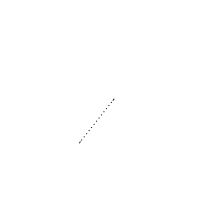
\includegraphics[width=4cm]{ressources/zoom-k3-slides.png}
              \end{center}
        \item <2-> attribuer à la fleur inconnue, la variété la plus présente parmi ses \emph{k} voisins.
    \end{itemize}
    \note{\textbf{k N}earest \textbf{N}eighbors}

\end{frame}
\subsection{Choix du k}
\begin{frame}
    \frametitle{Choix du k}

    \begin{center}
        \centering
        \includegraphics[width=8cm]{ressources/zoom-k3.png}
        \captionof{figure}{Détermination de l'iris (5.05, 1.5) pour $k = 3$}
        \label{IMG}
    \end{center}
\end{frame}
\begin{frame}

    \begin{center}
        \centering
        \includegraphics[width=8cm]{ressources/zoom-k7.png}
        \captionof{figure}{Détermination de l'iris (5.05, 1.5) pour $k = 7$}
        \label{IMG}
    \end{center}
    \note[item]{avantages de kNN: simple d'implémentation et résultats avec bon taux de réussite quand on a un gros échantillon}
    \note[item]{inconvénients: sensible au bruit (données mal étiquetées), sensible à l'échelle de chaque dimension}
\end{frame}
\begin{frame}
    \frametitle{}

    \begin{aretenir}[]
        Un bon choix de la valeur \textbf{k} est difficile a priori. Plusieurs tests permettent de déterminer la valeur la plus adaptée à l'étude en cours.
    \end{aretenir}
    \begin{aretenir}[Remarque]
        En pratique on partage les données en deux parties:
        \begin{itemize}
            \item les données d'entraînement,
            \item les données tests.
        \end{itemize}
        On teste différentes valeurs de k avec les données tests et on choisit la plus adaptée.
    \end{aretenir}
\end{frame}

\subsection{Calcul de la distance}
\begin{frame}
    \frametitle{Calcul de la distance}

    \begin{aretenir}[]
        Il existe plusieurs méthodes pour mesurer la distance entre l'élément étudié et son voisin:
        \begin{itemize}
            \item distance euclidienne,
            \item distance de Manhattan.
        \end{itemize}
    \end{aretenir}

\end{frame}
\begin{frame}
    $$d=\sqrt{(x_A-x_B)^2+(y_A-y_B)^2}$$
    \begin{center}
        \centering
        \includegraphics[width=6cm]{ressources/euclidienne.png}
        \captionof{figure}{distance euclidienne}
        \label{IMG}
    \end{center}
\end{frame}

\begin{frame}

    $$d=\lvert x_A-x_B\rvert+\lvert y_A-y_B\rvert$$
    \begin{center}
        \centering
        \includegraphics[width=6cm]{ressources/manhattan.png}
        \captionof{figure}{distance de Manhattan}
        \label{IMG}
    \end{center}
\end{frame}
\subsection{Implémentation}
\begin{frame}
    \frametitle{Implémentation}
    L'algorithme kNN peut s'écrire:
    \begin{itemize}
        \item Charger les données dans le programme.
        \item Choisir k.
        \item Stocker les mesures de la fleur inconnue.
        \item Calculer la distance euclidienne entre la fleur inconnue et tous les autres iris.
        \item Sélectionner les \emph{k} plus proches iris (en distance) de la fleur inconnue.
        \item Affecter la variété majoritaire  des \emph{k} plus proches iris (en distance) à la fleur inconnue.
    \end{itemize}


\end{frame}

\begin{frame}
    \frametitle{}

    \begin{activite}
        \begin{enumerate}
            \item Télécharger et extraire le dossier compressé \texttt{\textbf{iris-eleve.zip}} depuis le site \url{https://cviroulaud.github.io}
            \item Ouvrir le fichier \texttt{\textbf{data-iris.csv}} avec un tableur pour observer les données.
            \item Ouvrir le fichier \texttt{\textbf{iris-eleve.py}}


        \end{enumerate}
    \end{activite}

\end{frame}
\begin{frame}
    \frametitle{Correction}

    \begin{center}
        \begin{tabular}[]{|*{3}{c|}}
            \hline
            petal\_length & petal\_width & species \\
            \hline
            1.4           & 0.2          & setosa  \\
            \hline
            1.4           & 0.2          & setosa  \\
            \hline
            1.3           & 0.2          & setosa  \\
            \hline
        \end{tabular}
    \end{center}
    \note{3 attributs}
\end{frame}
\begin{frame}
    \frametitle{}
    \setcounter{compteuractivite}{2}

    \begin{activite}

        \begin{enumerate}
            \setcounter{enumi}{3}

            \item Compléter la fonction \texttt{\textbf{charger\_donnees}} en utilisant les informations du fichier \texttt{\textbf{csv}}.
            \item Compléter la fonction \texttt{\textbf{distance}} qui calcule le carré de la distance euclidienne entre deux points du plan.
            \item Compléter la fonction \texttt{\textbf{calculer\_distances}}.
            \item Compléter enfin la fonction \texttt{\textbf{trouver\_variete}}. Le dictionnaire \texttt{\textbf{compteur\_voisins}} compte le nombre d'apparitions de chaque variété parmi les \texttt{\textbf{k}} premiers voisins.
        \end{enumerate}
    \end{activite}

\end{frame}
\begin{frame}[fragile]
    \frametitle{Correction}
    \begin{center}
        \begin{lstlisting}[language=Python , basicstyle=\ttfamily\small, xleftmargin=0.2em, xrightmargin=-2em]
def charger_donnees(nom_fichier: str) -> list:
    fichier = open(nom_fichier, encoding="utf8")
    data_iris = csv.DictReader(fichier, delimiter=",")
    tab_iris = []
    # Pour chaque ligne de données
    for iris in data_iris:
        tab_iris.append(
            {"espece": iris["species"],
             "longueur": float(iris["petal_length"]),
             "largeur": float(iris["petal_width"])})

    fichier.close()
    return tab_iris
\end{lstlisting}
    \end{center}

\end{frame}
\begin{frame}[fragile]
    \frametitle{Correction}
    \begin{center}
        \begin{lstlisting}[language=Python , basicstyle=\ttfamily\small, xleftmargin=0.2em, xrightmargin=-3em]
def distance(connu: dict, inconnu: dict) -> float:
    return (connu["longueur"]-inconnu["longueur"])**2 + \
        (connu["largeur"]-inconnu["largeur"])**2
\end{lstlisting}
    \end{center}

\end{frame}
\begin{frame}[fragile]
    \frametitle{Correction}

    \begin{center}
        \begin{lstlisting}[language=Python , basicstyle=\ttfamily\small, xleftmargin=0.2em, xrightmargin=-2em]
def calculer_distances(donnees: list, inconnu: dict) -> list:
    distances = []
    for iris in donnees:
        # iris est un dictionnaire
        d = distance(iris, inconnu)
        # stocke la distance pour cet iris
        distances.append((iris["espece"], d))

    # trie les iris en fonction de la distance
    distances.sort(key=lambda fleur: fleur[1])
    return distances
\end{lstlisting}
    \end{center}

\end{frame}
\begin{frame}[fragile]
    \frametitle{Correction}
    \begin{center}
        \begin{lstlisting}[language=Python , basicstyle=\ttfamily\small, xleftmargin=0.2em, xrightmargin=-2em]
def trouver_variete(k: int, distances: list) -> str:
    # compte le nombre d'occurences de chaque variété
    compteur_voisins = {}
    for i in range(k):
        # espèce de l'iris de rang i
        nom = distances[i][0]
        # vérifie si l'espèce a déjà été référencée
        if nom in compteur_voisins:
            compteur_voisins[nom] += 1
        else:
            compteur_voisins[nom] = 1    
\end{lstlisting}
        \captionof{code}{Début de la fonction \textbf{\texttt{trouver\_variete}}}
    \end{center}

\end{frame}
\begin{frame}[fragile]
    \frametitle{}

    \begin{center}
        \begin{lstlisting}[language=Python , basicstyle=\ttfamily\small, xleftmargin=0.2em, xrightmargin=-2em]
    # recherche la variété avec la plus grande valeur dans compteur_voisins
    maxi = 0
    nom_maxi = 0
    for nom, quantite in compteur_voisins.items():
        if quantite > maxi:
            maxi = quantite
            nom_maxi = nom

    return nom_maxi
\end{lstlisting}
        \captionof{code}{Fin de la fonction \textbf{\texttt{trouver\_variete}}}
        \label{CODE}
    \end{center}

\end{frame}
\begin{frame}

    \begin{activite}
        Tester la fonction avec $k=3$ puis $k=7$, pour l'iris inconnu de mesures:
        \begin{itemize}
            \item longueur: 5,1
            \item largeur: 1,55
        \end{itemize}
    \end{activite}

\end{frame}
\begin{frame}[fragile]
    \frametitle{}

    \begin{center}
        \begin{lstlisting}[language=Python , basicstyle=\ttfamily\small, xleftmargin=0.2em, xrightmargin=-2em]
k = 3
inconnu = {"espece": "inconnu", 
            "longueur": 5.1, 
            "largeur": 1.55}

varietes = charger_donnees("data-iris.csv")
distances_cible = calculer_distances(varietes, inconnu)
variete = trouver_variete(k, distances_cible)

print("La variété est", variete)
\end{lstlisting}
    \end{center}

\end{frame}
\begin{frame}
    \frametitle{Code complet}

    Le code complet est accessible \href{https://cviroulaud.github.io/premiere/algorithmique/knn/iris/scripts/iris-correction.zip}{ici}.

\end{frame}
\end{document}